\usepackage{etex} %эта магическая херь избавляет от переполнения регистров TeX а!!!

\mode<article>{\usepackage{fullpage}}
\mode<presentation>{
    \usetheme{Madrid}
    \useoutertheme{shadow}
} 

\usepackage[utf8]{inputenc}
\usepackage[russian]{babel}
\usepackage{indentfirst}
\usepackage{graphicx}

\usepackage{amsmath}
\usepackage{amsfonts}
\usepackage{amsthm}
%\usepackage{algorithm}
%\usepackage{algorithmic}

%\usepackage[all]{xy}

\date{Лекция по дисциплине <<методы и средства защиты компьютерной информации>> (\today)}
\author[М.~М.~Шихов]{Михаил Шихов \\ \texttt{\underline{m.m.shihov@gmail.com}}}

%%для рисования графов пакетом xy-pic
%\entrymodifiers={++[o][F-]}

%%для псевдокода алгоритмов (algorithm,algorithmic)
%\renewcommand{\algorithmicrequire}{\textbf{Вход:}}
%\renewcommand{\algorithmicensure}{\textbf{Выход:}}
%\renewcommand{\algorithmiccomment}[1]{// #1}
%\floatname{algorithm}{Псевдокод}

%\setbeamercolor{alerted text}{fg=-green} %gyan, blue, green, -green

\title[Аутентификация: <<что знает>>, <<что имеет>>]{Методы аутентификации.\\ Признаки <<что знает>>, <<что имеет>>}

\newcommand{\Prv}{\textit{Д}}
\newcommand{\Ver}{\textit{П}}

\begin{document}


%титул и содержание статьи
\mode<article>{\maketitle\tableofcontents}

%титул и содержание презентации
\frame<presentation>{\titlepage}
\begin{frame}<presentation>
    \frametitle{Содержание}
    \tableofcontents
\end{frame}


\section{Аутентификация}


\begin{frame}
\frametitle{Аутентификация}
\begin{definition}%theorem, lemma, proof, corollary, example
\alert{Аутентификация} --- это проверка подлинности
\end{definition}
Аутентификация может быть произведена на основе проверки следующих признаков.
\begin{enumerate}
    \item \alert{Something you know (Что знает)}.
    \item \alert{Something you have (Что имеет)}.
    \item Something you are (Чем является).
    \item Something you can (Что умеет).
\end{enumerate}
Далее сосредоточим внимание на первых двух признаках.
\end{frame}


\begin{frame}
\frametitle{Аутентичность}
Возникает необходимость в аутентификации всех компонент информационной системы: 
\begin{itemize}
    \item персонала;
    \item клиентов (их автоматизированных систем);
    \item поставшиков (их автоматизированных систем);
    \item программных и программно-аппаратных средств;
    \item данных.
\end{itemize}
После аутентификации тот или иной компонент называют \alert{аутентичным}. В отношении сообщения, например, аутентичность=целостность+принадлежность.
\end{frame}


Аутентификацию можно провести в отношении различных компонент информационной системы: пользователей, аппаратных и программных средств, данных. Например, можно проверить подлинность пользователя, идентификатора, чип-карты, сообщения, сервера, клиента и т.д.

Чаще всего термин <<аутентификация>> употребляется в отношении проверки подлинности идентификатора пользователя или сервера информационных услуг. Компонент, прошедший аутентификацию называют \emph{аутентичным}, доверенным. Так например, аутентичным называют сообщение, для которого гарантированы фундаментальные свойства целостности и принадлежности.


\begin{frame}
\frametitle{Действующие лица}
\begin{figure}
    \begin{center}
        \mode<presentation>{ 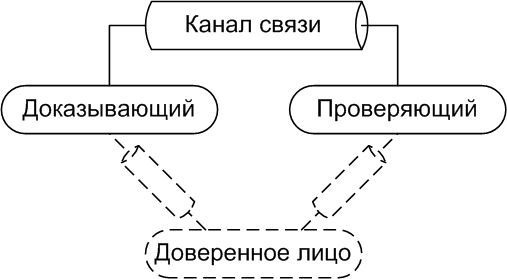
\includegraphics[width=.6\textwidth]{pict/actors} }
        \mode<article>{ 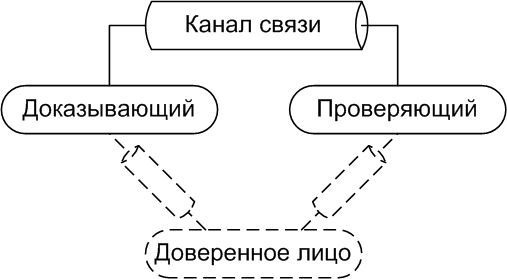
\includegraphics[width=.8\textwidth]{pict/actors} } 
    \end{center}
    \caption{Действующие лица}\label{pict:actors}
\end{figure} 
\mode<article>{См. рисунок \ref{pict:actors}}
Атакован злоумышленником может быть любой компонент приведенной схемы. 
\end{frame}


Действующие лица: доказывающая сторона, проверяющая сторона и канал связи. Возможно наличие третьей, доверенной стороны, с которой возможно общение по общему или выделенному каналу связи. Полагаться на то, что канал связи будет безопасным в процессе аутентификации, увы, нельзя. Например, кабель клавиатуры, с которой вводится пароль является источником электромагнитных излучений, которые могут быть перехвачены. Якобы безопасный канал связи, создаваемый вами, когда вы шепчете соседу на ушко секреты, таковым является только в том случае, если на вас не направлен параболический микрофон.


\begin{frame}
\frametitle{Классификация протоколов аутентификации}
\begin{definition}%theorem, lemma, proof, corollary, example
\alert{Протокол связи} --- это формализованное описание форматов сообщений и правил обмена ими между участниками (абонентами). Протокол определяет \alert{синтаксис}, \alert{семантику} и \alert{синхронизацию} общения абонентов.
\end{definition}

Протоколы аутентификации могут быть классифицированы по следующим признакам:
\begin{itemize}
    \item По количеству факторов доказательства подлинности: однофакторные; двухфакторыные (TFA, 2FA); многофакторные.
    \item По необходимости взаимного доказательства: односторонняя; взаимная.
    \item По наличию доверенной третьей стороны.
\end{itemize}
\end{frame}


\begin{itemize}
    \item По количеству факторов доказательства подлинности: однофакторные; двухфакторыные; многофакторные. Однофакторые используют какой либо один признак, например ввод пароля. Двухфакторые используют два независимых фактора для аутентификации. Примером могут служить банковские карты: для успешной аутентификации необходимо не только \emph{обладать} (<<Что имею>>) картой, а также \emph{знать} (<<Что знаю>>) PIN-код. Многофакторные могут использовать значительное количество факторов, например, аутентификация в банке: проверка по голосу, сетчатке глаза, ввд пароля, двойные ключи, и т.д.
    \item По необходимости взаимного доказательства: односторонняя; взаимная. В ряде случаев необходима взаимная аутентификация, когда, оба участника являются одновременно и доказывающей и проверяющей стороной.
    \item По наличию доверенной третьей стороны. Иногда удобнее возложить задачу аутентификации отдельной доверенной подсистеме. Примером может служить протокол Kerberos, в котором используется доверенный сервер аутентификации.
\end{itemize}


\begin{frame}
\frametitle{Характеристики протоколов аутентификации, которые следует учитывать при выборе}
Существует большое количество протоколов аутентификации. Выбор подходящего среди них --- непростая задача. Наиболее существенными характеристиками являются следующие.
\begin{itemize}
    \item Наличие взаимной аутентификации.
    \item Вычислительная эффективность.
    \item Коммуникационная эффективность.
    \item Наличие доверенной стороны.
    \item Формальные гарантии безопасности.
\end{itemize}
\end{frame}


\section{Аутентификация на основе паролей}


\subsection{Парольная система}


Правильная парольная аутентификация. Система не должна давать информации о: правильности ввода логина; длине используемого пароля. Идентификация и аутентификация должны происходить одной транзакцией, по завершении которой нужно выдать информацию лишь о том, успешна она или нет (потому \#2). 

\begin{frame}
    \frametitle{Какая парольная система лучше?}
    В каждом случае пользователь будет вводить данные (логин/пароль) в следующей последовательности: \alert{fail}/\alert{fail}; \alert{good}/\alert{fail}; \alert{good}/\alert{good}.
    
    \begin{columns}
        \column{.28\textwidth}
            \begin{block}{\#1}
                \begin{tabular}[c]{l}
                    login:\alert{fail}\\
                    login failed!\\
                    login:\alert{good}\\
                    password:\\
                    bad password!\\
                    login:\alert{good}\\
                    password:\\
                    login successful!\\
                    gooduser\$\\
                    ~
                \end{tabular}
            \end{block}
        
        \column{.28\textwidth}
            \begin{block}{\#2}
                \begin{tabular}[c]{l}
                    login:\alert{fail}\\
                    password:\\
                    login failed!\\
                    login:\alert{good}\\
                    password:\\
                    login failed!\\
                    login:\alert{good}\\
                    password:\\
                    login successful!\\
                    gooduser\$
                \end{tabular}
            \end{block}
            
        \column{.28\textwidth}
            \begin{block}{\#3}
                \begin{tabular}[c]{l}
                    login:\alert{fail}\\
                    password:\alert{****}\\
                    login failed!\\
                    login:\alert{good}\\
                    password:\alert{****}\\
                    login failed!\\
                    login:\alert{good}\\
                    password:\alert{****}\\
                    login successful!\\
                    gooduser\$
                \end{tabular}
            \end{block}
    \end{columns}
\end{frame}


Парольная защита --- наиболее популярный в мире информационных технологий способ аутентификации.


\begin{frame}
\frametitle{Структура парольной системы}
Состав парольной системы обычно таков:
\begin{itemize}
    \item пользовательский интерфейс аутентификации;
    \item пользовательский интерфейс администратора;
        \mode<article>{(к нему можно получить доступ только после взаимодействия с интерфейсом аутентификации)}
    
    \item база данных учетных записей пользователей;
    \mode<article>{(обычно содержащая соответствия: имя пользователя $\rightarrow$ внутрисистемный идентификатор, информация для проверки подлинности пароля, соль и т.д.)}
    
    \item компоненты базовой схемы аутентификации (программно-аппаратные модули доказывающего и проверяющего, канал связи)
    \item программный интерфейс сопряжения с другими подсистемами безопасности (например, с подсистемой контроля доступа).
\end{itemize}
\end{frame}


Аутентификации, то есть проверке подлинности пароля пользователя предшествует поиск введенного имени пользователя в базе учетных записей --- идентификация. Внутрисистемный идентификатор пользователю будет назначен после успешной аутентификации.


Обычно парольная система — передний край обороны всей системы и потому чаще всех остальных подсистем подвергается атакам.

\begin{frame}
\frametitle{Угрозы парольной системе}
Можно выделить следующие угрозы:
\begin{itemize}
    \item пoдcмaтpивaниe;
    \item пpeднaмepeнная пepeдaча пapoля влaдeльцeм дpyгoмy лицy;
    \item зaxвaт бaзы учетных записей пapoльнoй cиcтeмы (компрометация);
    \item xpaнeниe пapoля в дocтyпнoм мecтe;
    \item oбнapyжeниe и иcпoльзoвaниe oшибoк, дoпyщeнныx нa стaдии paзpaбoтки;
    \item вывeдeниe из cтpoя пapoльнoй cиcтeмы;
    \item и т.д.
\end{itemize}
\end{frame}


\begin{frame}
\frametitle{Атаки на парольную систему}
Атакован может быть любой компонент парольной системы. Наиболее распространенные атаки:
\begin{itemize}
    \item подбор грубой силой (brute-force, полный перебор) в интерактивном режиме или минуя интерфейс;
    \item словарные атаки (в том числе с применением эвристик);
    \item взлом базы учетных записей;
    \item пассивный и активный перехват;
    \item воспроизведение;
    \item внeдpeниe пpoгpaммныx зaклaдoк;
    \item и т.д.
\end{itemize}
\end{frame}


Закладка --- программа, эмулирующая пользовательский интерфейс аутентификации и производящая хищение учетных данных. Например, в Windows предусмотрена защита от закладок: событие для комбинации клавиш Ctrl+Alt+Del не может быть перехвачено прикладной программой, а потому можно доверять интерфейсу, появляющемуся в момент нажатия этой комбинации.


\begin{frame}
\frametitle{Оценка стойкости пароля}
Для оценки стойкости пароля важное значение имеют следующие характеристики.
\begin{itemize}
    \item Мощность алфавита паролей $A$.
    \item Длина пароля $L$.
    \item Мощность пространства паролей $S$ ($S = A^L$).
    \item Скорость подбора паролей $V$.
    \item Срок действия пароля (задает промежуток времени, по истечении которого пароль должен быть обязательно сменен) $T$.
    \item Вероятность подбора пароля в течение его срока действия (подбор продолжается непрерывно в течение всего срока действия пароля) $P$.
\end{itemize}
\end{frame}

\begin{frame}
    \frametitle{Оценка минимальной длина пароля}
    
    \begin{example}[Длина пароля]
        Определить минимальную длину пароля в соответствии с заданной вероятностью подбора $P$ в течение его срока действия $T$. Пусть $P=10^{-6}$, $T=1$ неделя, скорость интерактивного подбора паролей $V=10$ [паролей/мин], а мощность алфавита $A=33$.
    \end{example}
    \begin{example}[Длина пин-кода]
        Определить минимальную длину пин-кода, если даётся три подряд идущих попытки неправильного ввода. Гарантировать ту же вероятность подбора, что и в предыдущем задании при мощности алфавита $A=10$.
    \end{example}
\end{frame}

\[P=\frac{V\cdot T}{S}=\frac{V\cdot T}{A^L}\]
откуда и выражаем:
\[L=\log_{A}\frac{V\cdot T}{P}.\]
Ответ: $L\simeq 8.417184358$.


Для оценки стойкости ПИН кода (вероятности угадывания) вводится параметр <<количество попыток угадывания>> $N$. В этом случае $P=\frac{N}{S}=\frac{N}{A^L}$.


\begin{frame}[allowframebreaks]
\frametitle{Требования к паролям, устанавливаемые политикой информационной безопасности}
\begin{itemize}
    \item Устaнoвлeниe минимaльнoй длины пapoля.
    \mode<article>{Уcлoжняeт зaдaчy злoyмышлeнникa пpи пoпыткe пoдcмoтpeть пapoль или пoдoбpaть пapoль мeтoдoм <<грубой силы>>.}
    
    \item Иcпoльзoвaниe в пapoлe paзличныx гpyпп cимвoлoв.
    \mode<article>{Уcлoжняeт зaдaчy злoyмышлeнникa пpи пoпыткe пoдoбpaть пapoль мeтoдoм <<грубой силы>>.}
    
    \item Проверка и отбраковка пароля по словарю.
    \mode<article>{Усложняет задачу злоумышленника при попытке подобрать пароль по словарю.}
    
    \item Установление максимального срока действия пароля.
    \mode<article>{Усложняет задачу злоумышленника по подбору паролей методом грубой силы, в том числе без непосредственного обращения к системе защиты (режим off-line).}
    
    \item Установление минимального срока действия пароля.
    \mode<article>{Препятствует попыткам пользователя заменить пароль на старый после его смены по предыдущему требованию.}
    
    \item Ведение журнала истории паролей.
    \mode<article>{Препятствует попыткам пользователя установить возможно скомпрометированный пароль.}
    
    \item Применение эвристического алгоритма, бракующего пароли на основании данных журнала истории.
    \mode<article>{Усложняет задачу злоумышленника при попытке подобрать пароль по словарю или с использованием эвристик.}
    
    \item Ограничение числа попыток ввода пароля.
    \mode<article>{Препятствует интерактивному подбору паролей злоумышленником.}
    
    \item Поддержка режима принудительной смены пароля пользователя.
    \mode<article>{Обеспечивает эффективность требования, ограничивающего максимальный срок действия пароля.}
    
    \item Использование задержки при вводе неправильного пароля.
    \mode<article>{Препятствует интерактивному подбору паролей злоумышленником.}
    
    \item Запрет на выбор пароля самим пользователем и автоматическая генерация паролей.
    \mode<article>{Исключает возможность подобрать пароль по словарю. Если алгоритм генерации паролей не известен злоумышленнику, последний может подбирать пароли только методом <<грубой силы>>}
    
    \item Принудительная смена пароля при первой регистрации пользователя в системе.
    \mode<article>{Защищает от неправомерных действий системного администратора, имеющего доступ к паролю в момент создания учетной записи.}

\end{itemize}
\end{frame}


\begin{frame}
\frametitle{Как создать хороший пароль?}
Мало придумать пароль --- еще нужно \alert{запомнить}. Некоторые применимые способы (по возрастанию стойкости) приведены ниже.

\begin{enumerate}
    \item \alert{Алогичное словосочетание.} Например: <<круглокуб>>, <<водогрыз>>, <<клювоходик>>, <<пятнокрылыйпоплетун>>, <<ежпушистыйполосатый>>, <<фотомотобыстротих>> и т.д.
    \item \alert{Контркультурная фраза}\footnote{Хороший пример в романе <<Фальшивые зеркала>>, \copyright~С.В. Лукьяненко, 1999. Не реклама!}. Фраза <<Арестован Хомяк, 1 Мая загнавший 3-х Котов на Березу>> легко преобразуется в пароль, например: <<АрХо1Маза3КонаБе>>.
    \item \alert{Зубрежка}. Создать монстра, наподобие <<73gp8mFk13sRT5x>> и запомнить, испльзуя мнемотехники\footnote{Можно предложить метод ассоциаций, или метод Цицерона}.
\end{enumerate}

Конечно, полученные пароли, можно <<посолить>> по своему вкусу.
\mode<article>{Например, добавить неалфавитные символы, цифры, менять регистры, набирать в другой раскладке и т.д.}

\end{frame}


\subsection{Аутентификация на основе хеш функций}


Одним из важнейших инструментов для решения этой задачи является криптографическая хеш-функция. Отличия криптографической хеш-функции от обычной заключаются в том, что эта функция обладает стойкостью к коллизии первого и второго рода. Обычная хеш-функция $H$ преобразует информационную последовательность символов $M$ (в частном случае бит) произвольной длины в последовательность $h$ фиксированной длины $H:M\rightarrow h$. Вычисляется хеш-функция очень быстро и обычно используется для ускорения поиска символьных имен в таблицах переменных при компиляции/интерпретации или для проверки целостности информации (как контрольная сумма).

Количество всех возможных аргументов $M$ функции $H$ огромно (так как ограничений на длину $M$ нет, то можно сказать, что количество всех аргументов бесконечно). Количество же значений $h$ конечно и относительно невелико. В случае кодирования битами $2^{L(h)}$, где $L(h)$ --- длина битовой цепочки на выходе хеш-функции. Таким образом, на одно и то же значение $h$ отображается огромное множество аргументов $M$. Сей факт называется \emph{коллизией}, когда $H(M_1 )=H(M_2)$, но $M_1\neq M_2$.
Криптографическая хеш-функция $H$ необратима: вычислительно невозможно найти для заданного значения $h$ хеш-функции $H$ её аргумент $M$, такой, что $H(M)=h$.

\begin{frame}
\frametitle{Аутентификация}
\begin{definition}%theorem, lemma, proof, corollary, example
\alert{Хеш-функция} $H:M\rightarrow h$ --- это функция, преобразующая последовательность символов $M$ произвольной длины в последовательность $h$ фиксированной длины. $h=H(M)$.
\end{definition}
\alert{Криптографическая} хеш-функция обладает стойкостью следующих родов.
\begin{enumerate}
    \item Стойкость к коллизиям \alert{первого} рода: для заданного сообщения $M_1$ вычислительно невозможно подобрать сообщение $M_2$, такое, что $H(M_1)=H(M_2)$.
    \item Стойкость к коллизиям \alert{второго} рода: вычислительно невозможно сформировать пару сообщений $M_1,M_2$, таких, что $H(M_1)=H(M_2)$.
\end{enumerate}
\end{frame}

Криптографические хеш-функции, используемые на практике: sha-1, sha-2, sha-3. Не используйте MD5!!!

Конечно, сравнение введенного пароля с паролем, хранимым в базе паролей на проверяющей стороне по очевидным причинам не может использоваться. Но на практике продолжает использоваться! Банальный пассивный перехват компрометирует парольную систему.

\begin{frame}
\frametitle{Базовая схема парольной аутентификации}
\framesubtitle{Защита от пассивного перехвата}
\begin{figure}
    \begin{center}
        \mode<presentation>{ 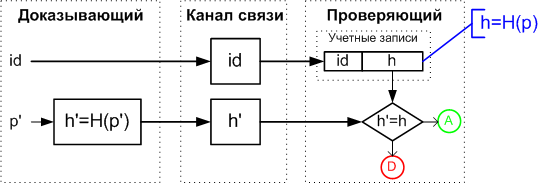
\includegraphics[width=.9\textwidth]{pict/pwdhashbase} }
        \mode<article>{ 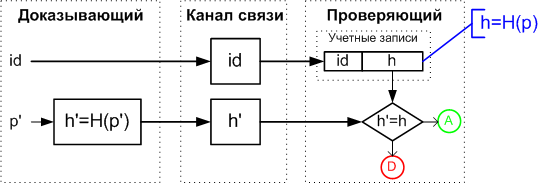
\includegraphics[width=.8\textwidth]{pict/pwdhashbase} } 
    \end{center}
    \caption{Защита от пассивного перехвата}\label{pict:pwdhashbase}
\end{figure} 
\mode<article>{См. рисунок \ref{pict:pwdhashbase}}
\end{frame}


Действительно, если у злоумышленника есть возможность вести только пассивный перехват, то схема гарантирует защиту. Зная h невозможно вычислить p. Но вот если злоумышленник имеет прямой доступ к каналу, минуя интерфейс ввода пароля на стороне доказывающего, очевидно, что от атаки повтором данная схема не защищает.

Также схема неустойчива к словарной атаке. Допустим, что злоумышленник располагает словарем популярных паролей. Ему достаточно выполнить предобработку словаря, вычислив хеш $H(p)$ для каждого пароля $p$ в словаре. Допустим, что злоумышленник похитил базу паролей. Ему достаточно сравнить полученные хеши для словаря с хешами в похищенной базе паролей. Наверняка там будет несколько совпадений. А стало быть злоумышленник выяснил для некоторых пользователей их пароли. Затруднить жизнь злоумышленнику можно, <<посолив>> пароль (т.е. добавив к паролю случайное значение salt: $H(p+salt)$), в следующей схеме в качестве соли используется id.


\begin{frame}
\frametitle{Базовая схема парольной аутентификации}
\framesubtitle{Защита от пассивного перехвата и словарной атаки}
\begin{figure}
    \begin{center}
        \mode<presentation>{ 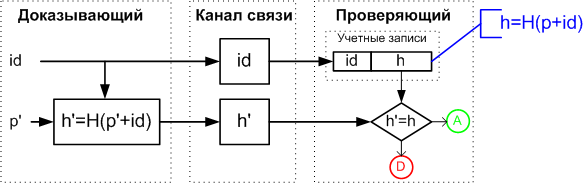
\includegraphics[width=.9\textwidth]{pict/pwdhashbasedict} }
        \mode<article>{ 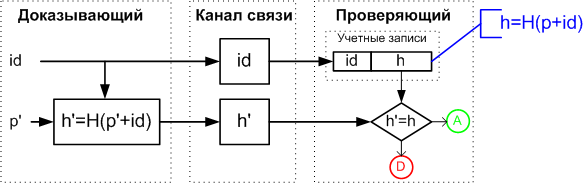
\includegraphics[width=.8\textwidth]{pict/pwdhashbasedict} } 
    \end{center}
    \caption{Защита от пассивного перехвата и словарной атаки}\label{pict:pwdhashbasedict}
\end{figure} 
\mode<article>{См. рисунок \ref{pict:pwdhashbasedict}}
\end{frame}


Теперь допустим, что злоумышленник крадет хеш из базы паролей. Ему достаточно просто сформировать необходимые данные в канале для предыдущих схем. Защищаясь от записи в канал, формируем проверочные хеши на стороне проверяющего. Увы, пароль в этом случае придется передавать в канал в открытом виде.


\begin{frame}
\frametitle{Базовая схема парольной аутентификации}
\framesubtitle{Защита от компрометации проверяющего}
\begin{figure}
    \begin{center}
        \mode<presentation>{ 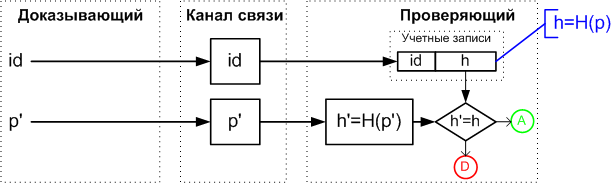
\includegraphics[width=.9\textwidth]{pict/pwdhashcompr} }
        \mode<article>{ 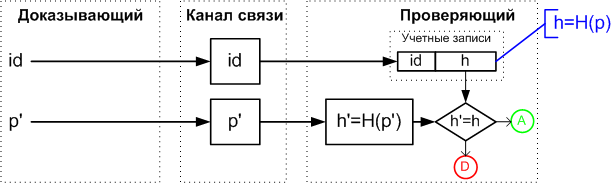
\includegraphics[width=.8\textwidth]{pict/pwdhashcompr} } 
    \end{center}
    \caption{Защита от компрометации проверяющего}\label{pict:pwdhashcompr}
\end{figure} 
\mode<article>{См. рисунок \ref{pict:pwdhashcompr}}
\end{frame}


Теперь защитим предложенную схему от словарной атаки.


\begin{frame}
\frametitle{Базовая схема парольной аутентификации}
\framesubtitle{Защита от компрометации проверяющего и словарной атаки}
\begin{figure}
    \begin{center}
        \mode<presentation>{ 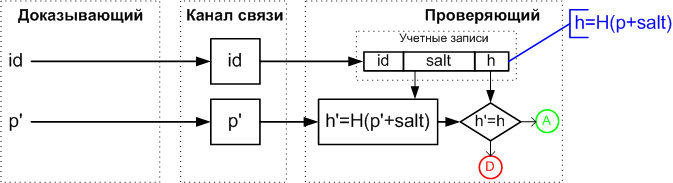
\includegraphics[width=.9\textwidth]{pict/pwdhashcomprdict} }
        \mode<article>{ 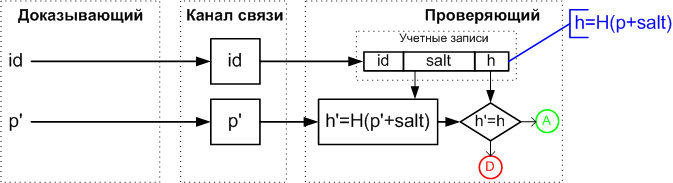
\includegraphics[width=.8\textwidth]{pict/pwdhashcomprdict} } 
    \end{center}
    \caption{Защита от компрометации проверяющего и словарной атаки}\label{pict:pwdhashcomprdict}
\end{figure} 
\mode<article>{См. рисунок \ref{pict:pwdhashcomprdict}}
\end{frame}

Параметр salt (соль) добавляется для затруднения словарной атаки. Допустим, что у злоумышленника имеется словарь в $N$ записей, чтобы выполнить предвычисления <<соленых>> хешей ему нужно будет выполнить $N\cdot 2^L(salt)$ вычислений, то есть в $2^L(salt)$ больше.


Скомбинируем два варианта для получения стойкого к компрометациям проверяющего, словарной атаке и пассивному перехвату варианта.

\begin{frame}
\frametitle{Базовая схема парольной аутентификации}
\framesubtitle{Защита от компрометации проверяющего, пассивного перехвата и словарной атаки}
\begin{figure}
    \begin{center}
        \mode<presentation>{ 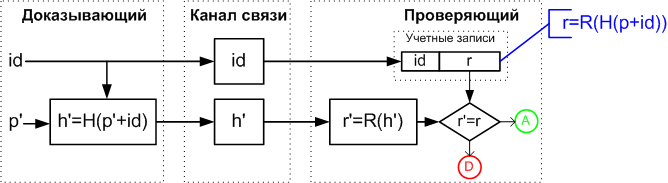
\includegraphics[width=.9\textwidth]{pict/pwdhashtotal} }
        \mode<article>{ 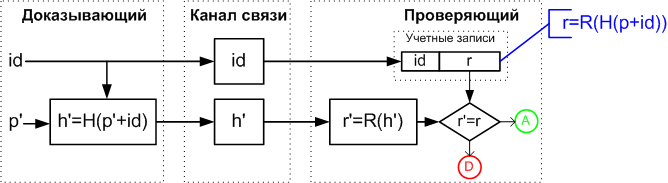
\includegraphics[width=.8\textwidth]{pict/pwdhashtotal} } 
    \end{center}
    \caption{Защита от компрометации проверяющего, пассивного перехвата и словарной атаки}\label{pict:pwdhashtotal}
\end{figure} 
\mode<article>{См. рисунок \ref{pict:pwdhashtotal}}
\end{frame}


К сожалению, ни одна из перечисленных схем не является стойкой к атаке воспроизведения. Приведем стойкий к этой атаке вариант.


\begin{frame}
\frametitle{Базовая схема парольной аутентификации}
\framesubtitle{Защита от атаки повторного воспроизведения}
\begin{figure}
    \begin{center}
        \mode<presentation>{ 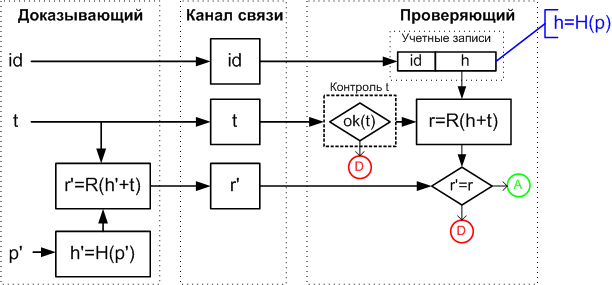
\includegraphics[width=.9\textwidth]{pict/pwdhashreplay} }
        \mode<article>{ 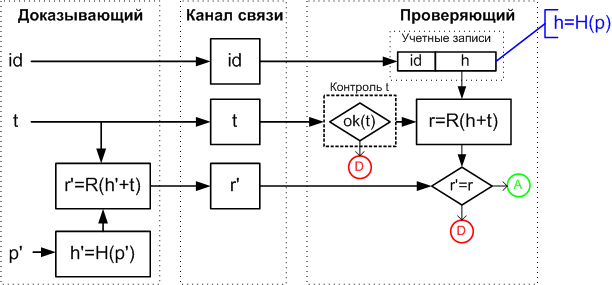
\includegraphics[width=.8\textwidth]{pict/pwdhashreplay} } 
    \end{center}
    \caption{Защита от атаки повторного воспроизведения}\label{pict:pwdhashreplay}
\end{figure} 
\mode<article>{См. рисунок \ref{pict:pwdhashreplay}}
\end{frame}

Увы, данная схема не является стойкой к компрометации проверяющего. Но эта схема приближает нас к идее одноразовых паролей!


\subsection{Одноразовые пароли}


Реализовать схему, стойкую к повторному воспроизведению можно просто: достаточно потребовать, чтобы пароль после использования менялся. Таким образом, злоумышленник, перехватив старый пароль, не будет знать, какой пароль будет использован в следующий раз.

\begin{frame}
\frametitle{Одноразовый пароль}
\begin{definition}%theorem, lemma, proof, corollary, example
Суть схемы \alert{одноразовых паролей} в том, что в каждом запросе на аутентификацию используется <<уникальный>> пароль.
\end{definition}
Схема успешно противостоит атакам повторного воспроизведения, что достигается за счет:
\begin{itemize}
    \item Использования общего списка случайных паролей для доказывающей и проверяющей стороны (и механизма их синхронизации).
    \item Общий генератор псевдослучайной последовательности с секретным разделяемым seed.
    \item Механизм временных меток и безопасной службы единого времени.
\end{itemize}
Элемент, гарантирующий уникальность (например, случайное число или метка времени), называется в литературе \alert{nonce}.
\end{frame}


 Чтобы избавить администратора и пользователя от головной боли, можно предложить следующую схему, основанную на схеме защиты от повторного воспроизведения (см. \ref{pict:pwdhashreplay}). При этом вводится понятие аппаратного ключа (кеу), который недоступен для программных средств и его установка требует физического вмешательства в аппаратную часть. Ключ прошит как в интерфейсе доказывающего, так и на проверяющей стороне. Это разделяемый секрет, компрометация которого технически затруднена (например, его невозможно похитить у проверяющего не имея физического доступа к аппаратуре).

\begin{frame}
\frametitle{Схема одноразовых паролей}
\framesubtitle{Одноразовый пароль на аппаратном ключе (key)}
\begin{figure}
    \begin{center}
        \mode<presentation>{ 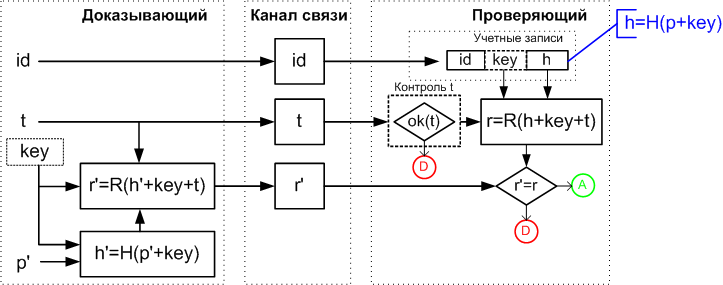
\includegraphics[width=.9\textwidth]{pict/pwduniqkey} }
        \mode<article>{ 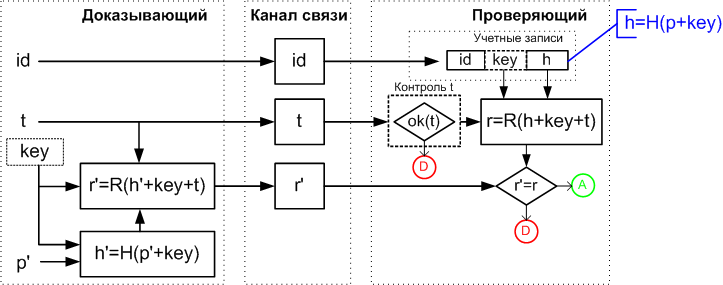
\includegraphics[width=.8\textwidth]{pict/pwduniqkey} } 
    \end{center}
    \caption{Одноразовый пароль на аппаратном ключе (key)}\label{pict:pwduniqkey}
\end{figure} 
\mode<article>{См. рисунок \ref{pict:pwduniqkey}}
\end{frame}


Введение ключа решает в некотором роде проблему компрометации проверяющего --- ключ (key) не может быть скомпрометирован одновременно с базой учетных записей (на рис. \ref{pict:pwduniqkey} ключ выделен пунктиром), а потому подделка данных в канале без знания ключа невозможна. nonce параметр t может и не передаваться, если используется общий генератор псевдослучайной последовательности, счетчик или метки времени.


Другой оригинальной схемой на хеш-функциях явлеется аутентификация s-key. Изобретатель данной схемы --- Лесли Лэмпорт (1981). Схему также иногда называют \emph{односторонней цепочкой хеширования} (\emph{one-way hash chain}).


\begin{frame}
\frametitle{Схема одноразовых паролей s-key}
\framesubtitle{one-way hash chain, схема Лэмпорта}
Рекурсивно последовательность s-key паролей $\{p_0,\ldots, p_N\}$ определяется так:
    \[
        \begin{cases}
            p_N = H(S), N > 0\\
            p_i = H(p_{i+1}), 0 \leq i < N
        \end{cases}
    \]
Тогда, например
    \[
        p_0 = \underbrace{ H(H(\cdots H(S)\cdots )) } _ {N + 1}.
    \]

\alert{Секрет} $S$ генерируется случайным образом. Выбирается нужное \alert{количество попыток аутентификации} $N$, не требующих смены $S$. Проверяющая строна запоминает $N$, пару $\langle p_0,0\rangle$ и уничтожает $S$. Доказывающая сторона запоминает $N, S$ и $i=1$.
\end{frame}


\begin{frame}
\frametitle{Схема одноразовых паролей s-key}
\framesubtitle{Процесс аутентификации}
Процесс аутентификации на i-м шаге выглядит следующим образом.
\begin{enumerate}
    \item<1-> $\Prv\rightarrow\Ver$: $\Prv,\langle p_i,i\rangle$. 
    Доказывающий ($\Prv$), зная секрет $S$, легко вычислит $p_i$ для любого $i$. Проверяющий ($\Ver$), получив пару $\langle p_i,i\rangle$ извлекает по идентификатору {$\Prv$} пару $\langle p_j,j\rangle$ из своей базы паролей. Далее проверяющий проверяет условие \[R=(j+1==i)\land (p_j==H(p_i)),\] определяющее успешность аутентификации. Если $R==true$, то проверяющий запомпнает в базе паролей для $\Prv$ пару $\langle p_i,i\rangle$.
    
    \item<2-> $\Prv\leftarrow\Ver$: $R$. 
    Доказывающий, пройдя аутентификацию ($R==true$), увеличивает на $1$ счетчик $i$: $i=i+1$.
\end{enumerate}
\uncover<3->{При достижении $i==N$ требуется \alert{новая инициализация} протокола.}
\end{frame}


Схема одноразовых паролей s-key создает для злоумышленника следующие проблемы:

\begin{enumerate}
    \item Скомпометировать проверяющего нет возможности, так как секрет $S$ им не хранится. Все что доступно, это уже использовавшийся ранее пароль, который не даст информации о следующем, и сам уже не будет использован.
    \item Как пассивный, так и активный перехват не дадут эффекта, так как, перехваченный $\langle p_i,i\rangle$ уже не будет использован, а угадать следующую пару $\langle p_{i+1},i+1\rangle$ нет возможности, так как для этого нужно реверсировать хеш-функцию: $p_i = H(p_{i+1})$.
    \item Злоумышленник может рассчитывать, что при условии использования функции $H$ долгое время многими участниками некоторые последовательности начнут пересекаться. Свести эти надежды на нет (т.е. уменьшив в $2^k$ раз) можно k-битной солью.
\end{enumerate}


\section{Аутентификация: <<что знает>>, <<что имеет>>}


Парольная защита является частным случаем данной темы. Все, что будет сказано далее отчасти справедливо и для нее.


\subsection{Запрос-ответ}


\begin{frame}
\frametitle{Запрос-ответ}
\framesubtitle{challenge-response. Общая схема}
\begin{figure}
    \begin{center}
        \mode<presentation>{ 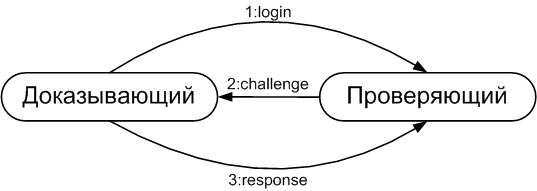
\includegraphics[width=.9\textwidth]{pict/chalresp} }
        \mode<article>{ 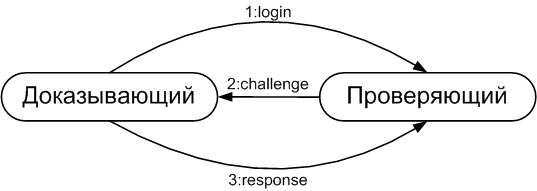
\includegraphics[width=.8\textwidth]{pict/chalresp} } 
    \end{center}
    \caption{Общая схема протокола <<Запрос-ответ>>}\label{pict:chalresp}
\end{figure} 
\mode<article>{См. рисунок \ref{pict:chalresp}}
\end{frame}


\begin{frame}
\frametitle{Запрос-ответ}
\framesubtitle{Реализация на хеш-функциях. Односторонняя}
\begin{figure}
    \begin{center}
        \mode<presentation>{ 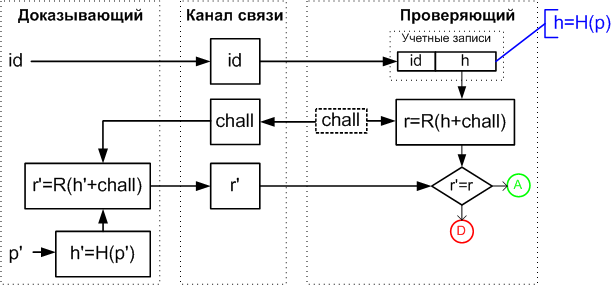
\includegraphics[width=.9\textwidth]{pict/chalresphash} }
        \mode<article>{ 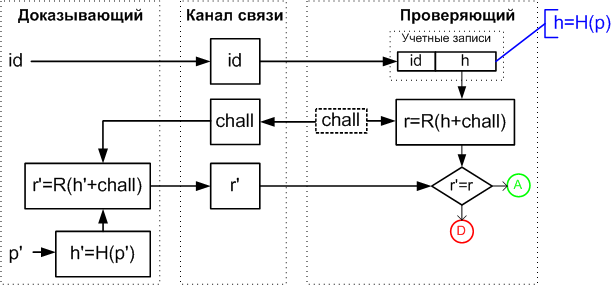
\includegraphics[width=.8\textwidth]{pict/chalresphash} } 
    \end{center}
    \caption{Реализация протокола <<запрос-ответ>> на хеш-функциях}\label{pict:chalresphash}
\end{figure} 
\mode<article>{См. рисунок \ref{pict:chalresphash}}
\end{frame}


\begin{frame}
\frametitle{Запрос-ответ}
\framesubtitle{Реализация на хеш-функциях. Обоюдная}
Реализацию протокола можно сделать обоюдной:
\begin{enumerate}
    \item $\Prv\rightarrow\Ver$: \Prv.
    \item $\Ver\rightarrow\Prv$: $r_{\Ver}$. \label{enum:chalresp2}

    \mode<article> {
    $r_{\Ver}$ --- случайное число, созданное $\Ver$.
    }
    
    \item $\Prv\rightarrow\Ver$: $r_{\Prv}, R(H(p')+r_{\Prv}+r_{\Ver}+\Ver)$.

    \mode<article> {
    $r_{\Prv}$ --- случайное число, созданное $\Prv$. Проверяющий извлекает из сообщения $r_{\Prv}$, и рассчитывает $R(H(p)+r_{\Prv}+r_{\Ver}+\Ver)$ по паролю $p$ из базы учетных записей и переданному на шаге \ref{enum:chalresp2} запросу $r_{\Ver}$. Если результат совпал со вторым блоком сообщения --- доказывающий аутентичен!
    }
    
    \item $\Prv\rightarrow\Ver$: $R(H(p)+r_{\Prv}+r_{\Ver}+\Prv)$.
    
    \mode<article> {
    Чтобы убедиться в том, что проверяющий аутентичен, доказывающий вычисляет значение по той же формуле, подставив данные своей стороны. Если результаты совпали, то проверяющий аутентичен!
    }
\end{enumerate}


\end{frame}


\subsection[Криптографическая аутентификация]{Криптографические протоколы аутентификации}


\begin{frame}
\frametitle{Базовая схема передачи информации}
\begin{figure}
    \begin{center}
        \mode<presentation>{ 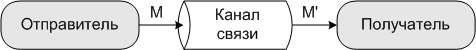
\includegraphics[width=.8\textwidth]{pict/basechannel} }
        \mode<article>{ 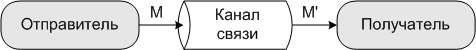
\includegraphics[width=.8\textwidth]{pict/basechannel} }
    \end{center}
    \caption{Базовая схема передачи информации}\label{pict:basechannel}
\end{figure} 
\mode<article>{См. рисунок \ref{pict:basechannel}}

Можно выделить следующие виды \alert{каналов связи}:
\begin{itemize}
    \item \alert{Секретный} гарантирует конфиденциальность, целостность и принадлежность M;
    \item \alert{Аутентичный} гарантирует только целостность и принадлежность M;
    \item \alert{Открытый} не гарантирует ничего в отношении M.
\end{itemize}

\end{frame}


Криптографическая защита --- это защита на \emph{уровне представления} информации\footnote{Уровней доступа к информации, как известно, четыре: носителя, средств взаимодействия с носителем, \emph{представления}, содержания (смысла)}. Далее мы рассмотрим криптографические схемы, направленные на защиту конфиденциальности.

Конфиденциальность – это, как уже известно, недоступность третьим лицам. Первые два лица – это источник (отправитель) и получатель информации в процессе передачи информации. Третье лицо – злоумышленник, для которого передаваемая информация должна оставаться недоступной. Выход – ограничить доступ третьих лиц к каналу передачи информации, либо перекодировать информацию так, чтобы её восприятие стало им недоступно. Такое перекодирование называется шифрованием. Об особенностях шифрования и поговорим далее.

Разработкой методов шифрования (в том числе) занимается криптография. Исследованием творений криптографии на стойкость занимается криптоанализ. Оба направления, криптография и криптоанализ, объединяются в единую науку – криптологию.

Методы шифрования разделяют на два вида: симметричные и асимметричные. Очень важным условием для существования самой возможности шифрования является наличие \emph{секрета}.


\begin{frame}
\frametitle{Схемы шифрования}
\framesubtitle{Симметричная схема}
\begin{figure}
    \begin{center}
        \mode<presentation>{ 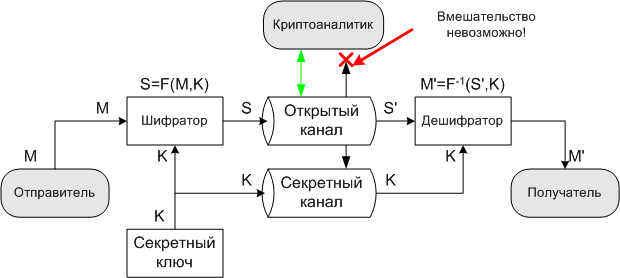
\includegraphics[width=.8\textwidth]{pict/symmcipher} }
        \mode<article>{ 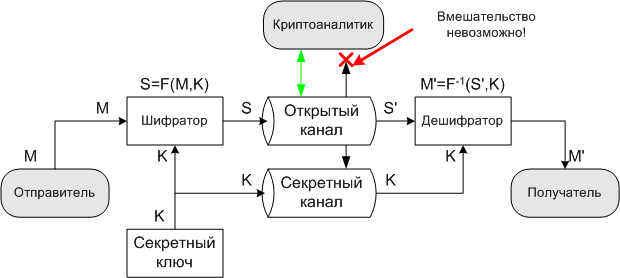
\includegraphics[width=.8\textwidth]{pict/symmcipher} }
    \end{center}
    \caption{Симметричная схема шифрования}\label{pict:symmcipher}
\end{figure} 
\mode<article>{См. рисунок \ref{pict:symmcipher}}
\end{frame}


Исходное сообщение (информация M) отправитель преобразует с помощью шифратора в шифротекст $S$. Для этого преобразования шифратором используется функция $F:M,K\rightarrow S$ , вторым аргументом которой является секретная информация – ключ $K$. Ключ $K$ известен только отправителю и получателю, они и только они  разделяют этот секрет. Злоумышленник, который в данной схеме назван криптоаналитиком, секретом $K$ овладеть не может \emph{по определению}! С выхода шифратора шифротекст $S$ передается через открытый канал получателю. При этом шифротекст может получить и криптоаналитик. Более того, криптоаналитик даже может внести изменения в шифротекст, и до получателя дойдет уже не $S$, а $S'$.  Получатель  восстанавливает из шифротекста $S'$ исходное сообщение $M'$ с помощью дешифратора. Дешифратором, используется функция $F^{-1}:S,K\rightarrow M$ , позволяющая выполнить обратное преобразование: $F^{-1}(F(M,K),K)=M$ . Без знания ключа восстановить из шифротекста $S$ исходное сообщение $M$ практически невозможно. Даже зная функции $F$  и $F^{-1}$ , криптоаналитик, не зная ключа $K$, не в силах восстановить сообщение. В этом, к слову, и заключается важнейшее правило криптографии, сформулированное голландским криптологом Керкхоффом: стойкость шифра должна зависеть только от секретности ключа.

Криптоаналитик может испортить жизнь законным участникам обмена, исказив или подменив шифротекст. Увы, осмысленных изменений без знания ключа ему не сделать! Более того, если до шифрования в сообщение $M$ была внесена избыточность с целью защиты целостности, то факт вмешательства будет обнаружен получателем после дешифрования и заработает стратегия повторной передачи.

Следует обратить внимание, что в схеме используется \emph{секретный канал}. Спрашивается, раз есть секретный канал для передачи ключей, то почему же не использовать это сокровище для передачи сообщений? Увы, секретный канал слишком дорог. Использовав его один раз для обмена секретным ключом, законные отправитель и получатель теперь могут организовать секретный канал передачи на основе любого открытого, что гораздо дешевле.

\emph{Симметричным} шифр назван потому, что один и тот же ключ применяется как для шифрования, так и для дешифрования.
Существует множество симметричных шифров. Современный симметричный шифр стоек и математически обоснован. Стандартом в настоящее время является шифр AES, в девичестве Rijndael. Активно используется и модификация бывшего стандарта DES --- шифр DES3. Впрочем, помимо стандартов существует множество проверенных временем шифров, которые могут использоваться в системах защиты информации. Использовать недавно созданный \emph{гениальным} автором \emph{сверхстойкий} шифр нужно лишь в целях информационного самоубийства.


\begin{frame}
\frametitle{Схемы шифрования}
\framesubtitle{Ассиметричная схема}
\begin{figure}
    \begin{center}
        \mode<presentation>{ 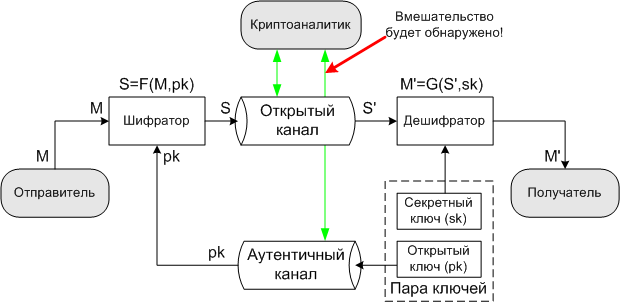
\includegraphics[width=.8\textwidth]{pict/asymmcipher} }
        \mode<article>{ 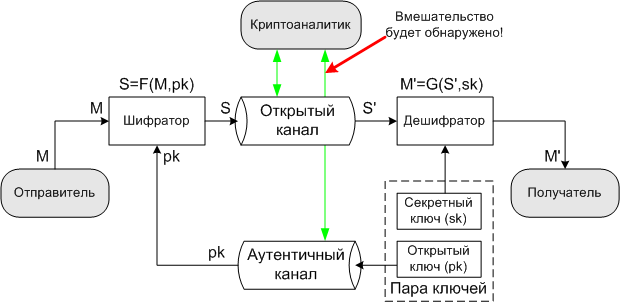
\includegraphics[width=.8\textwidth]{pict/asymmcipher} }
    \end{center}
    \caption{Асимметричная схема шифрования}\label{pict:asymmcipher}
\end{figure} 
\mode<article>{См. рисунок \ref{pict:asymmcipher}}
\end{frame}


Особенность ассиметричного шифра заключается в том, что для шифрования и дешифрования используются разные ключи $(sk, pk)$. Пара ключей $\langle sk, pk\rangle$ генерируется получателем относительно легко. Один из этой пары ключей будет открытым $pk$ (public key), и может быть передан неограниченному числу отправителей. Ключ $sk$, парный открытому, держится отправителем в секрете: $sk$ – secret(private) key. Важнейшей особенностью схемы является то, что, зная открытый ключ $pk$, вычислить по нему секретный $sk$ практически невозможно. Шифрование осуществляется с помощью открытого ключа, дешифрование с помощью секретного. Более того, восстановить из шифротекста исходное сообщение без знания секретного ключа практически невозможно: $G(F(M, pk), sk)=M$. Криптоаналитик может завладеть открытым ключом (впрочем великодушный получатель может сразу послать ему копию), но дешифровать сообщения он не сможет. Ему остается только слать получателю зашифрованные проклятия. Расшифровать сообщения может только обладатель секрета $sk$.

Шифруют все, расшифровывает один.

Внимательный читатель обратил внимание на то, что открытый ключ $pk$ передается по аутентичному каналу. Да, открытый канал для передачи открытого ключа $pk$ нельзя использовать ни в коем случае! Представте себе, что злоумышленник сгенерировал свою пару $\langle sk1, pk1\rangle$, перехватил $pk$, когда он передавался отправителю, и вместо перехваченного ключа послал отправителю от имени получателя свой открытый ключ $pk1$. Отправитель, будучи уверен в том, что $pk1$ – это открытый ключ получателя, зашифрует для него сообщение. Злоумышленник перехватит его, расшифрует на своем $sk1$, внесет необходимые поправки, зашифрует перехваченным $pk$ и отошлет получателю. Отправитель и получатель отныне общаются через двуликого Януса. Как же быть? Нужно использовать \alert{аутентичный} канал. Аутентичный канал гарантирует целостность и принадлежность информации. Получив данные по такому каналу, вы уверены в том, что информация в процессе передачи не была испорчена (целостность), и в том, что вы получили её именно от того, от кого и рассчитывали получить (принадлежность). Аутентичный канал дороже открытого, но дешевле секретного. Можно использовать секретный канал вместо аутентичного, хуже не будет, а в ряде случаев это просто необходимо.

Распространенные и проверенные временем схемы ассиметричного шифрования: RSA (факторизация), Диффи-Хеллмана (дискретное логарифимирование), алгоритмы на основе эллиптических кривых ECES.


\begin{frame}
\frametitle{Обозначения}
\begin{itemize}
    \item Абоненты обозначаются большими буквами: $A$, $B$,\ldots
    \item Nonce обозначается $n$. $n_A$ --- nonce созданный абонентом $A$.
    \item Mетка времени: $t$. $t_A$ --- метка времени $A$.
    \item Случайное число: $r$. $r_A$ --- случайное число, созданное $A$.
    \item Ключ симметричной схемы, разделяемый $A$ и $B$: $k_{AB}$.
    \item Открытый ключ $A$: $pk_A$.
    \item Секретный ключ $A$: $sk_A$.
    \item Сертификат открытого ключа $pk_A$: $cert_A$.
    \item Конкатенация сообщений $M_1$ и $M_2$: $M_1, M_2$.
    \item Зашифрованное на ключе $k$ сообщение $M$: $\{M\}k$.
    \item Обмен. $A$ передает $B$ сообщение $M$: $A\rightarrow B:M$.
\end{itemize}
\end{frame}


\begin{frame}
\frametitle{Криптографическая аутентификация}
\framesubtitle{Симметричная схема. Запрос-ответ}
$\Prv$ --- доказывающий, $\Ver$ --- проверяющий.

\alert{Односторонняя:}
\begin{enumerate}
    \item $\Prv\rightarrow \Ver:\Prv$.
    \item $\Ver\rightarrow \Prv:r_{\Ver}$.
    \item $\Prv\rightarrow \Ver:\{\Ver, r_{\Ver}\}k_{\Prv\Ver}$.
\end{enumerate}

\alert{Обоюдная:}
\begin{enumerate}
    \item $\Prv\rightarrow \Ver:\Prv$.
    \item $\Ver\rightarrow \Prv:r_{\Ver}$.
    \item $\Prv\rightarrow \Ver:\{\Ver, r_{\Prv}, r_{\Ver}\}k_{\Prv\Ver}$.
    \item $\Ver\rightarrow \Prv:\{r_{\Prv}, r_{\Ver}\}k_{\Prv\Ver}$.
\end{enumerate}
\end{frame}


\begin{frame}
\frametitle{Криптографическая аутентификация}
\framesubtitle{Асимметричная схема. Запрос-ответ}
${\Prv}$ --- доказывающий, ${\Ver}$ --- проверяющий.

\alert{Односторонняя:}
\begin{enumerate}
    \item ${\Prv}\rightarrow {\Ver}:{\Prv}$
    \item ${\Ver}\rightarrow {\Prv}:\{r_{\Ver},{\Ver}\}pk_{\Prv}$
    \item ${\Prv}\rightarrow {\Ver}:r_{\Ver}$
\end{enumerate}

\alert{Обоюдная} (Нидхема-Шредера):
\begin{enumerate}
    \item ${\Prv}\rightarrow {\Ver}:\{{\Prv},r_{\Prv}\}pk_{\Ver}$.
    \item ${\Ver}\rightarrow {\Prv}:\{{\Ver},r_{\Prv},r_{\Ver}\}pk_{\Prv}$.
    \item ${\Prv}\rightarrow {\Ver}:\{{\Prv},r_{\Ver}\}pk_{\Ver}$.
\end{enumerate}

\end{frame}


Как можно доверять тому, что открытый ключ $pk_{\Prv}$ принадлежит именно ${\Prv}$, а не другому лицу? Гарантии тому дает использование аутентичного канала в ассиметричной схеме. Но как создать подобный канал? Один из способов --- использовать сертификаты.

Далее рассмотрим аутентификацию, использующую сертификаты, для чего вначале обсудим схему цифровой подписи (ЭЦП) дающую гарантии целостности и принадлежности подписанной информации.

Кстати, федеральным законом об электронной  цифровой подписи, принятом в 2002 году, установлен юридический статус этому понятию. Цифровая подпись является доказательством в суде, как и рукописная подпись под бумажным документом. 


\begin{frame}
\frametitle{Цифровая подпись}
\begin{figure}
    \begin{center}
        \mode<presentation>{ 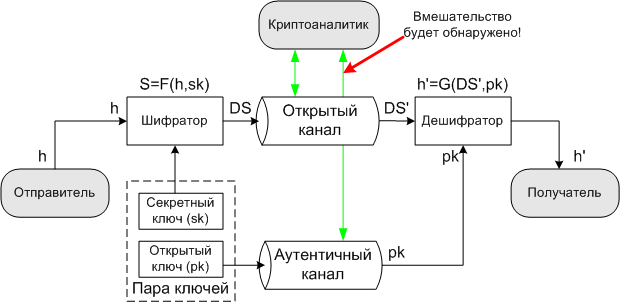
\includegraphics[width=.8\textwidth]{pict/signature} }
        \mode<article>{ 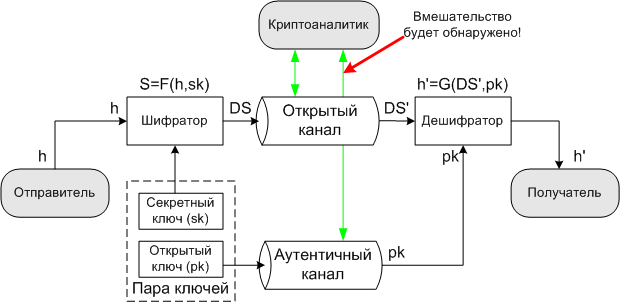
\includegraphics[width=.8\textwidth]{pict/signature} }
    \end{center}
    \caption{Цифровая подпись}\label{pict:signature}
\end{figure} 
\mode<article>{См. рисунок \ref{pict:asymmcipher}}
\end{frame}

Как видно, схема очень похожа на схему ассиметричного шифрования. Все сказанное в отношении схемы шифрования справедливо и для цифровой подписи, за исключением того, что обладателем секрета теперь является отправитель, и шифрование слепка сообщения $h$ производится на секретном ключе $sk$. Цифровой подписью называется результат шифрования слепка – $DS$. Без знания секретного ключа $sk$ шифрование невозможно. Любой желающий, имеющий открытый ключ $pk$, может дешифровать сообщение (проверить подпись).

Итак, зашифровать слепок может только один отправитель, а расшифровать --- любой желающий проверить подпись получатель.

При этом получатель, расшифровывающий $DS$ открытым ключом $pk$, уверен в том, что зашифровать слепок мог только обладатель секретного ключа $sk$ (парного открытому ключу $pk$). Уверен потому, что получил открытый ключ по аутентичному каналу.

Впрочем, пока не ясно, что представляет собой слепок $h$ сообщения $M$. Слепок может представлять собой копию сообщения $M$. Обычно и сообщение $M$, и его цифровая подпись DS передаются одним блоком $\langle M,DS\rangle$. Получателю достаточно расшифровать цифровую подпись $DS$ и сравнить с $M$. Совпадение будет означать, что полученное $M$ аутентично, так как гарантированы его целостность и принадлежность отправителю. Злоумышленник не сможет внести идентичные изменения в сообщение и в подпись, так как должен для этого вновь зашифровать измененную копию $M$, а это вычислительно невозможно без обладания секретным ключом $sk$. На практике (в целях экономии памяти) слепок $h$ формируется как результат хеширования сообщения с помощью криптографической хеш-функции: $h=H(M)$. Аналогично, сообщение $M$ и его цифровая подпись $DS=F(H(M), sk)$ передаются одним блоком $\langle M,DS\rangle$. Получатель, разделив, блок на части $M'$ и $DS'$, находит $H(M')$ и сравнивает с расшифрованной подписью $h'=G(DS', pk)$. Если эти величины равны --- сообщение $M$ аутентично. Злоумышленник, подделывая подпись, столкнется с необходимостью, либо зашифровать вычисленный им слепок $H(M')$ измененного сообщения $M'$ (что вычислительно невозможно без знания $sk$), либо подобрать такое осмысленное сообщение $M'$, чтобы оно давало такой же хеш, что и исходное $M$ (что вычислительно невозможно, так как $H$ обладает стойкостью к коллизиям первого рода).

Подписанному сообщению можно доверять в том случае, если вы доверяете подписавшему. Для того, чтобы быть уверенным в том, что открытый ключ ассиметричной схемы принадлежит пользователю ${\Prv}$, нужно, чтобы доверенное лицо подписало блок данных ${\Prv}, pk_{\Prv}$. Такой подписанный блок называется цифровым сертификатом открытого ключа. Сертифицированный открытый ключ становится <<аутентичным>>.

%QUEST: что такое аутентичный открытый ключ?

\begin{frame}
    \frametitle{Криптографическая аутентификация}
    \framesubtitle{Сертификаты, цифровая подпись}
    
    Согласно стандарту X.509 сертификат открытого ключа пользователя $A$ --- $cert_A$, содержит значения следующих параметров.
    \begin{enumerate}
        \item Уникальное имя пользователя $A$.
        \item Открытый ключ $A$: $pk_A$.
        \item Назначение ключа $pk_A$ (для шифрования или для проверки ЭЦП).
        \item Период действия сертификата (даты начала и конца периода)
        \item Серийный номер сертификата.
        \item Уникальное имя доверенного лица, подписавшего сертификат.
        \item Идентификатор и параметры алгоритма ЭЦП, которым подписан $cert_A$.
    \end{enumerate}
\end{frame}

Стандарт X.509 создан сектором ITU-T (Telecommunication Standardization Sector of ITU), который координирует стандарты для телекоммуникаций от имени ITU (International Telecommunication Union). Стандарт поддерживается группой IETF (RFC 1422,RFC 2459,).

Из рассмотренных ассиметричных схем видно, что открытые (и соответственно закрытые) ключи могут использоватся двояко: для шифрования и для дешифрования! Использовать открытый ключ, предназначенный для проверки ЭЦП для шифрования использовать нельзя!


\begin{frame}
\frametitle{Криптографическая аутентификация}
\framesubtitle{Пример сертификата}
\begin{figure}
    \begin{center}
        \mode<presentation>{ 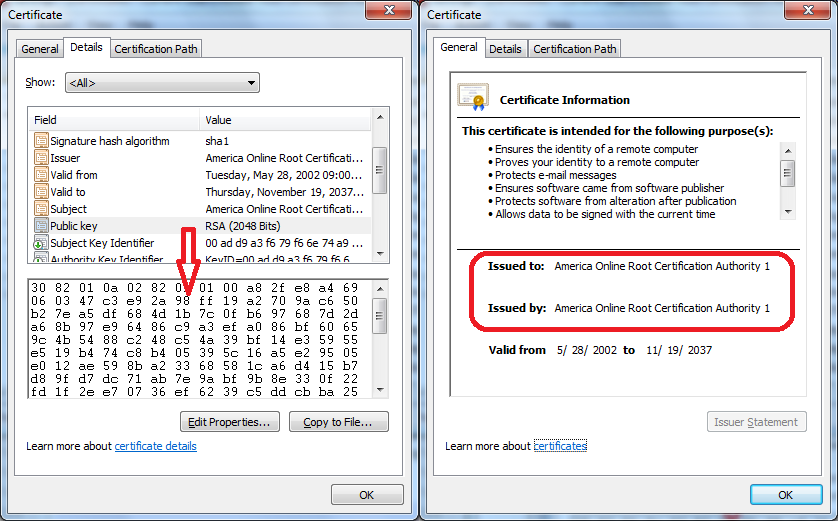
\includegraphics[width=.74\textwidth]{pict/certscreen} }
        \mode<article>{ 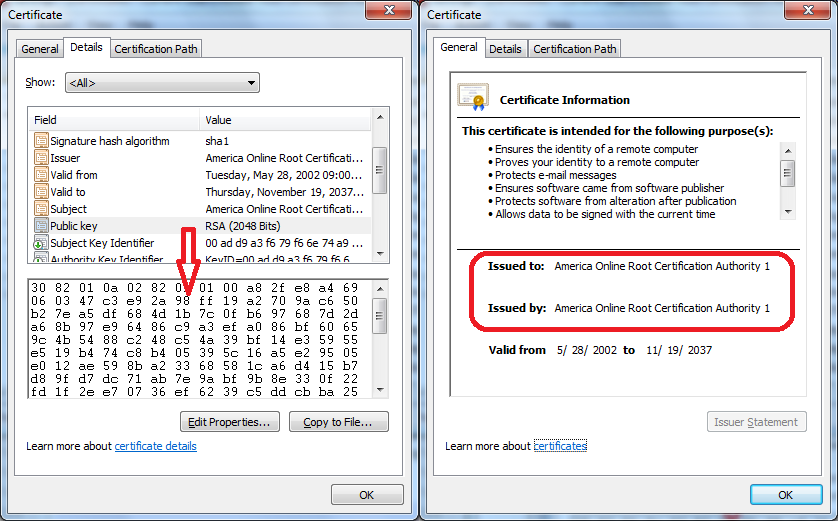
\includegraphics[width=.74\textwidth]{pict/certscreen} }
    \end{center}
    \caption{Пример сертификата}\label{pict:certscreen}
\end{figure}
\mode<article>{См. рисунок \ref{pict:certscreen}}
\end{frame}


В операционной системе обычно содержатся заранее установленные производителем сертификаты доверенных лиц, которым пользователь доверяет хотя бы в силу того, что приобрел данную ОС. О моделях построения центров сертификации (т.е. способов проверки подлинности сертификатов) поговорим на следующих лекциях.

На следующем слайде обратите внимание, что шифрование происходит на секретном ключе (цифровая подпись)!

\begin{frame}
    \frametitle{Криптографическая аутентификация}
    \framesubtitle{Сертификаты}
    
    ${\Prv}$ --- доказывающий, ${\Ver}$ --- проверяющий. $cert_{\Prv}=\{{\Prv}, pk_{\Prv},\ldots\}sk_C$, где $C$ --- доверенное лицо. 

    \alert{Односторонняя:}
    \begin{enumerate}
        \item ${\Prv}\rightarrow {\Ver}:{\Prv}$
        \item ${\Ver}\rightarrow {\Prv}:r_{\Ver}$
        \item ${\Prv}\rightarrow {\Ver}:cert_{\Prv},\{r_{\Ver},{\Ver}\}sk_{\Prv}$
    \end{enumerate}

    \alert{Обоюдная:}
    \begin{enumerate}
        \item ${\Prv}\rightarrow {\Ver}:{\Prv}$
        \item ${\Ver}\rightarrow {\Prv}:r_{\Ver}$
        \item ${\Prv}\rightarrow {\Ver}:cert_{\Prv},r_{\Prv},\{r_{\Prv},r_{\Ver},{\Ver}\}sk_{\Prv}$
        \item ${\Ver}\rightarrow {\Prv}:cert_{\Ver},\{r_{\Prv},r_{\Ver},{\Prv}\}sk_{\Ver}$
    \end{enumerate}
    \alert{Важно}:$\{M\}sk$ --- шифрование на \alert{закрытом} ключе, т.е. цифровая подпись
\end{frame}


\subsection[С нулевым разглашением]{Аутентификация с нулевым разглашением}


Протоколы с нулевым разглашением интерактивны и повторяемы (имитируемы).

\begin{frame}
\frametitle{Схемы с нулевым разглашением}
\framesubtitle{Концепция Zero-knowledge. Пещера Али-Бабы}
\begin{figure}
    \begin{center}
        \mode<presentation>{ 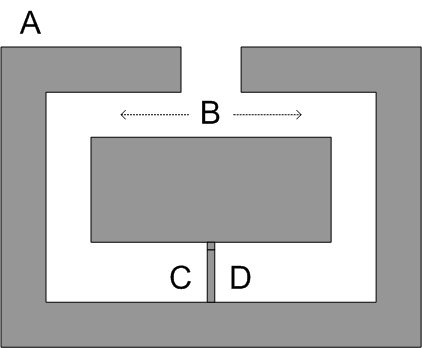
\includegraphics[width=.5\textwidth]{pict/zeroknowali} }
        \mode<article>{ 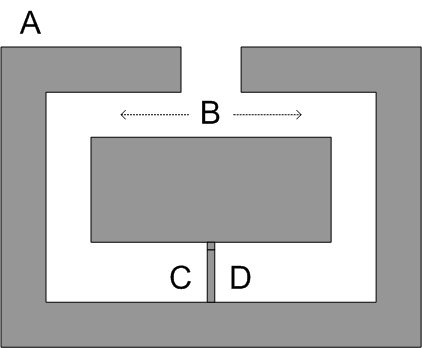
\includegraphics[width=.5\textwidth]{pict/zeroknowali} }
    \end{center}
    \caption{Пещера Али-Бабы}\label{pict:zeroknowali}
\end{figure}
\mode<article>{См. рисунок \ref{pict:zeroknowali}}
\end{frame}


Алгоритм итеративный и количество итераций определяется исходя из заданной вероятности  ложного подтверждения истинности обладания ключом. Одна успешная итерация.


\begin{enumerate}
    \item Проверяющий становится в точку A.
    \item Доказывающий проходит в пещеру и добирается до двери (оказывается в точке C или D). Проверяющий не видит, в какой из двух коридоров тот свернул.
    \item Проверяющий приходит в точку B и в соответствии со своим выбором просит доказывающего выйти из определенного коридора.
    \item Доказывающий, если нужно, открывает дверь ключом и выходит из названного проверяющим коридора.
\end{enumerate}
Проведя $N$ раундов, вероятность ошибочной аутентификации составит $P=\left(\frac{1}{2}\right)^N$.


\begin{frame}
    \frametitle{Схемы с нулевым разглашением}
    \framesubtitle{Изрморфизм графов}

    \mode<article>{Поиск изоморфизма графов относится к классу NP полных задач, т.е. не решаемых на компьтере при больших размерностях.}

    Доказывающий ${\Prv}$ знает об изоморфизме $\varphi$ общеизвестных графов $G_1$, $G_2$. Он тасует, например, граф $G_2$, получая граф $H$ ($H\neq G_1$) и подстановку $\psi$. \[G_{1}\xrightarrow{\varphi}G_2, G_2\xrightarrow{\psi}H, G_1\xrightarrow{\varphi\circ\psi}H\]

    \mode<article>{Для любого другого участника задача поиск изоморфизма между $G_1$ и $H$ или $G_2$ и $H$ также труден, как и поиск между $G_1$ и $G_2$. Тем не менее, не представляет никакой сложности создать пару изоморфных графов. Достаточно сгенерировать граф $G_1$ и создать для него изоморфный $G_2$, перенумеровав вершины.}

    Раунд протокола выглядит так:
    \begin{enumerate}
        \item ${\Prv}\rightarrow {\Ver}$: $H$
        \item ${\Ver}\rightarrow {\Prv}$: $k$. Где $k\in\{1,2\}$, т.е. просьба доказать изоморфизм $G_k$ и $H$.
        \item ${\Prv}\rightarrow {\Ver}$:
            \begin{enumerate}
                \item Если $k=1$, то передается $\varphi\circ\psi$, тк $G_1\xrightarrow{\varphi\circ\psi}H$
                \item Если $k=2$, то передается $\psi$, тк $G_2\xrightarrow{\psi}H$
            \end{enumerate}
    \end{enumerate}

    Раунд повторяется $N$ раз, причем каждый раз создается новый $H$ из графа $G_1$ или $G_2$.

\end{frame}


\section{Аутентичные сообщения}

Подводя итог, отметим, что в некоторых фазах протоколов важно дать гарантии аутентичности передаваемых сообщений. 

\begin{frame}
\frametitle{Аутентичные сообщения}
Базовые способы организации \alert{аутентичности} сообщения $M$. ${\Prv}$ --- доказывающий, ${\Ver}$ --- проверяющий.
\begin{itemize}
    \item Симметричная схема. ${\Prv}$ и ${\Ver}$ разделяют общий $k_{{\Prv}{\Ver}}$. Аутентичность сообщения $M$ гарантирует MAC (Message authentication code). MAC организуется с помощью хешей\footnote{В этом случае он называется HMAC (Hash-based MAC)} так:
    \[{\Prv}\rightarrow {\Ver}: M,H(M+k_{{\Prv}{\Ver}})\]
    \item Асимметричная схема. Гарант --- цифровая подпись. ${\Ver}$ обладает сертификатом $cert_{\Prv}$.
    \[{\Prv}\rightarrow {\Ver}: M,\{H(M)\}sk_{\Prv}\]
\end{itemize}
\end{frame}


\appendix %приложения


\begin{frame}
\frametitle{Источники}
Протоколы аутентификации можно найти в \cite{bib:smart:crypto,bib:shangin:protect}. Подробно об аутентификации на хеш-функциях в \cite{bib:chmora:crypto}. Описание парольных систем \cite{bib:shangin:protect, bib:tannen:os}. Протоколы с нулевым разглашением \cite{bib:smart:crypto,bib:shneir:applCrypto}.
\end{frame}


\begin{frame}[allowframebreaks]{Библиография}
    \bibliographystyle{gost780u}
    \bibliography{./../bibliobase}
\end{frame}


\end{document}